\documentclass[a4paper, 12pt]{book}
\usepackage[margin=2.5cm]{geometry}
\usepackage[italian]{babel}
%\usepackage{wrapfig}
\usepackage{graphicx}
\usepackage{hyperref}
\usepackage{subcaption}
\usepackage{amsmath}
\setlength{\parindent}{0pt}
\usepackage{parskip}
\usepackage[most]{tcolorbox}
\usepackage{soul}
\usepackage{xcolor}
\sethlcolor{yellow}
\usepackage{array}
\usepackage{booktabs}
\usepackage{tikz}
\usetikzlibrary{positioning}
\usepackage{longtable}
\usepackage{array}
\usepackage{fancyhdr}
\setlength{\headheight}{15pt}
\pagestyle{fancy}
\fancyhf{} % pulisce header e footer
\fancyhead[R]{\thepage} % numero pagina a destra nell'header
\renewcommand{\headrulewidth}{0pt} % (opzionale) elimina la riga orizzontale sotto l'header
\fancypagestyle{plain}{%
  \fancyhf{} % pulisce header e footer
  \fancyhead[R]{\thepage} % numero sempre in alto a destra
  \renewcommand{\headrulewidth}{0pt} % opzionale: niente linea
}
\setcounter{tocdepth}{3}

\title{\textbf{Elaborazione di segnali e immagini}}
\author{Mattia Nicolis}
\date{A.A. 2025-26}

\begin{document}

    \maketitle

    \tableofcontents
    \markboth{}{}

    %-------MODULO DI TEORIA------------------------------------
    %-------Prof: Manuele Bicego--------------------------------
    %-------Lez: mercoledì (8:30-11:30) [Aula Delta - Cav.3]----
    \chapter*{Teoria}
    \addcontentsline{toc}{chapter}{Teoria}

    \section*{Sistemi e segnali}
    \addcontentsline{toc}{section}{Sistemi e segnali}

    \begin{figure}[h]
      \centering
      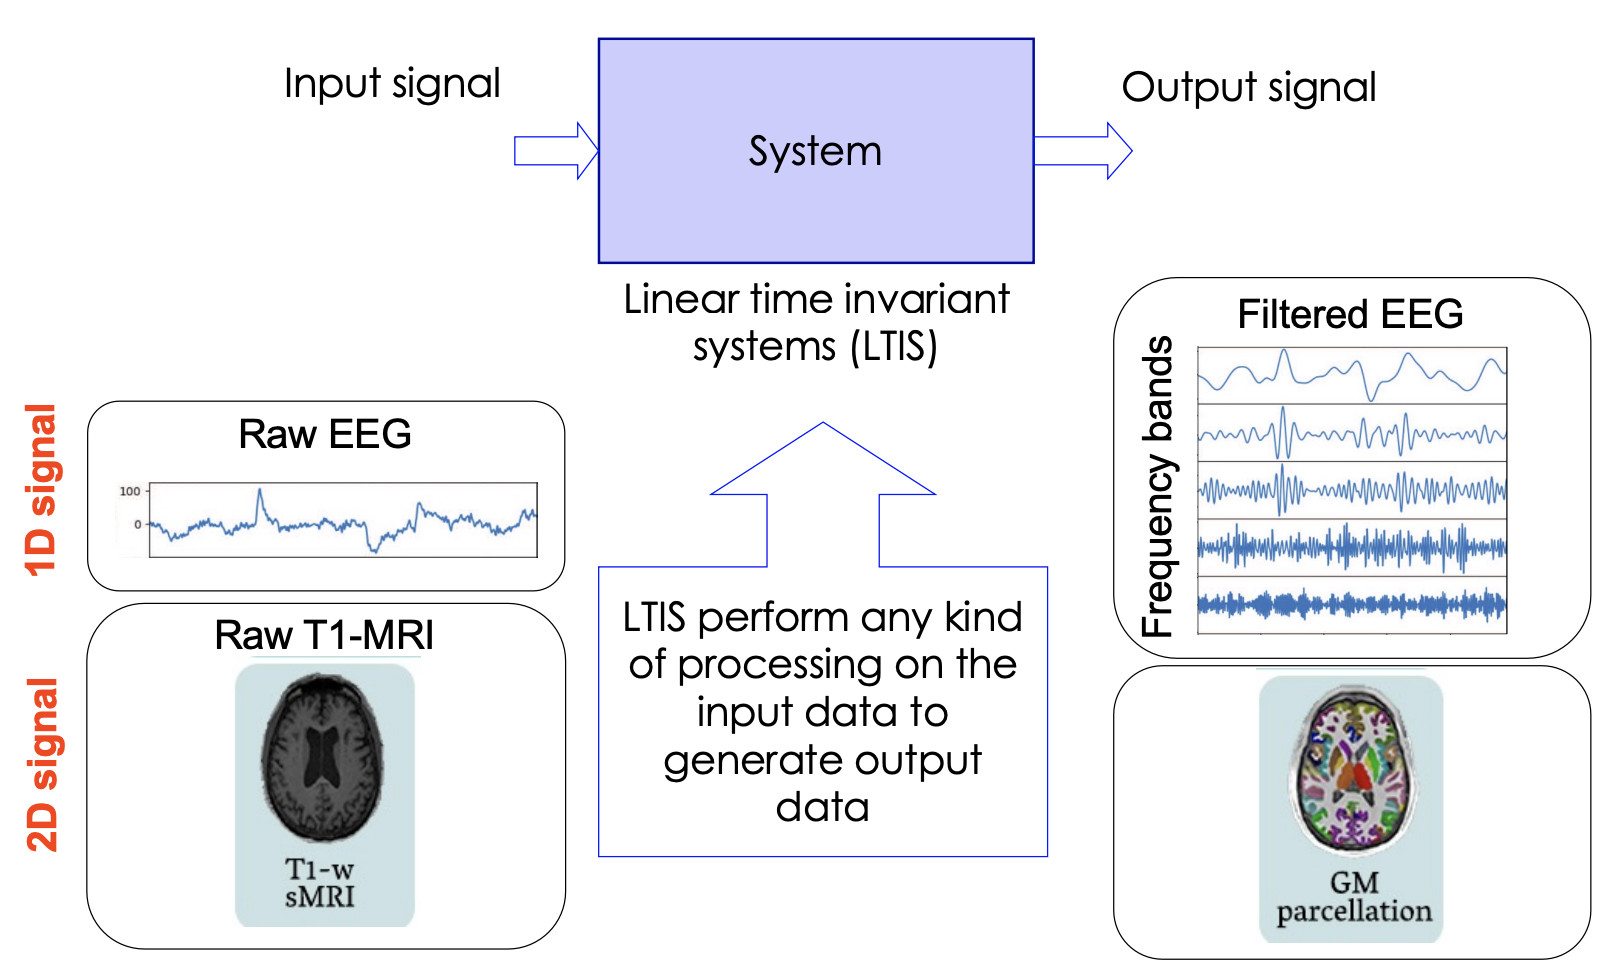
\includegraphics[width=0.6\textwidth, keepaspectratio]{foto/sistemi&segnali.png}
      \caption{sistema e segnali}
    \end{figure}

    \begin{tcolorbox}[
      colback=cyan!5!white,
      colframe=blue!50!black,
      title=\textbf{Segnale},
      coltitle=white,
      fonttitle=\bfseries,
      arc=3mm,
      boxrule=0.5pt,
      enhanced,
      breakable
    ]
      Un \textbf{segnale} è un \hl{insieme di dati o informazioni}.
    \end{tcolorbox}

    \vspace{2mm}

    Un segnale rappresenta qualsiasi tipo di variabile fisica soggetta a variazioni. 

    I segnali sono funzioni della variabile indipendente \textit{tempo} ($t$) o \textit{spazio} ($x, x = [x_1, x_2], x = [x_1, x_2, x_3]$).

    Sia la variabile indipendente che la variabile fisica possono essere scalari o vettoriali.

    Esempi di segnali:
    \begin{description}
      \item [segnali 1D]: segnale elettrocardiografico (EEG), segnale vocale, segnale audio
      \item [segnali 2D]: segnale immagine, segnale video 
      \item [segnali 3D]: segnale di dati volumetrici
    \end{description}

    \begin{figure}[h]
      \centering

      \begin{subfigure}[b]{0.45\textwidth}
        \centering
        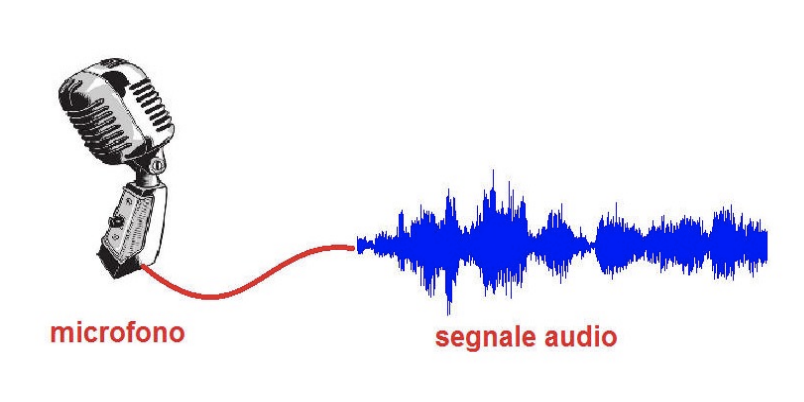
\includegraphics[width=\textwidth, height=3.8cm]{foto/segnale-audio.png}
        \caption{segnale 1D - segnale audio}
      \end{subfigure}
      \hfill
      \begin{subfigure}[b]{0.45\textwidth}
        \centering
        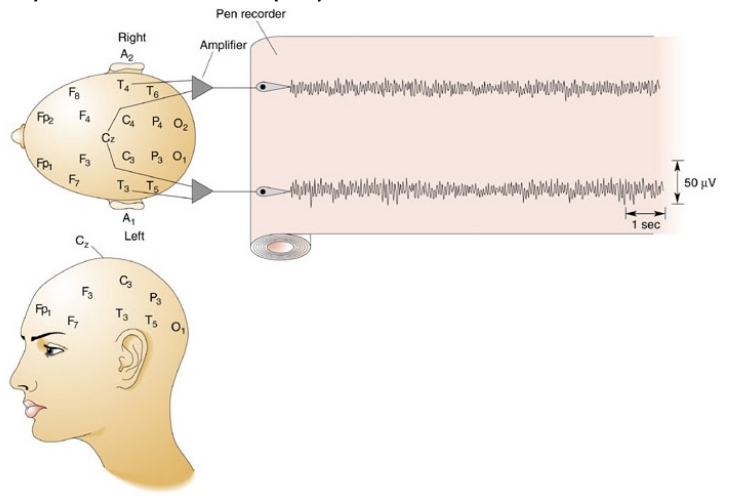
\includegraphics[width=\textwidth, height=3.8cm]{foto/segnale-elettrocardiogramma.png}
        \caption{segnale 1D - elettrocardiogramma}
     \end{subfigure}
    \end{figure}

    \
    
    Un segnale può essere elaborato da un \textbf{sistema}.

    \vspace{2mm}

    \begin{tcolorbox}[
      colback=cyan!5!white,
      colframe=blue!50!black,
      title=\textbf{Sistema},
      coltitle=white,
      fonttitle=\bfseries,
      arc=3mm,
      boxrule=0.5pt,
      enhanced,
      breakable
    ]
      Un \textbf{sistema} è un'\hl{entità che elabora un insieme di segnali (\textit{input}) per produrre un altro insieme di segnali (\textit{output})}.
    \end{tcolorbox}

    I sistemi processano i segnali per:
    \begin{itemize}
      \item estrarre informazioni
      \item consentire la trasmissione su canali con capacità limitata (JPEG, JPEG2000, codifica MPEG)
      \item migliorare la sicurezza sulle reti (crittografia, watermarking)
      \item migliorare la sicurezza sulle reti (crittografia, watermarking)
    \end{itemize}

    \begin{figure}[h]
      \centering
      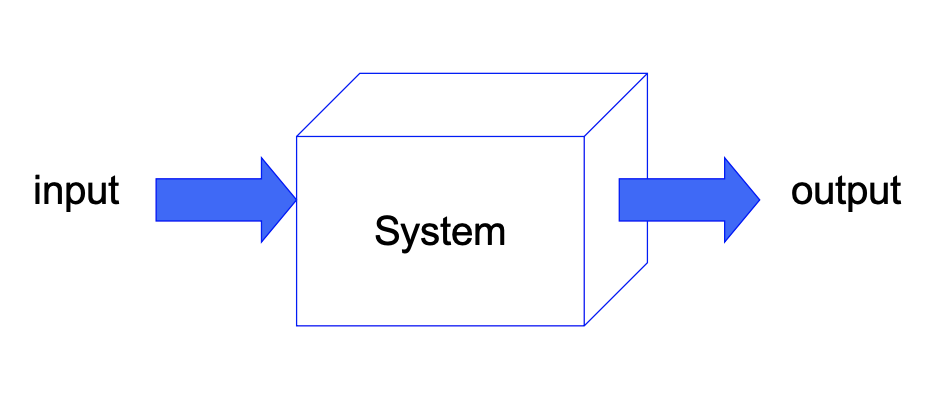
\includegraphics[width=0.6\textwidth, keepaspectratio]{foto/sistema.png}
      \caption{sistema}
    \end{figure}

    La funzione che collega l'uscita del sistema con il segnale di ingresso è chiamata \textbf{risposta all'impulso} $h(t)$ nel dominio del \textit{tempo} e \textbf{funzione di trasferimento} $H(\omega)$ nel dominio della \textit{frequenza}. 

    \subsection*{Classificazione dei segnali}
    \addcontentsline{toc}{subsection}{Classificazione dei segnali}
    I segnali possono essere di 4 tipologie:
    \begin{itemize}
      \item \textbf{segnali a tempo continuo} e \textbf{a tempo discreto}
      \item \textbf{segnali analogici} e \textbf{digitali}
      \item \textbf{segnali periodici} e \textbf{aperiodici}
      \item \textbf{segnali energetici} e \textbf{segnali di potenza}
      \item \textbf{segnali deterministici} e \textbf{probabilistci}
    \end{itemize}

    \subsubsection*{Segnali a tempo continuo e a tempo discreto}
    \addcontentsline{toc}{subsubsection}{Segnali a tempo continuo e a tempo discreto}







    %-------MODULO DI LABORATORIO-------------------------------
    %-------Prof: Menegaz Gloria--------------------------------
    %-------Lez: giovedì (15:30-18:30) [Aula A - Cav.1]---------
    \chapter*{Laboratorio}
    \addcontentsline{toc}{chapter}{Laboratorio}

\end{document}